\documentclass[12pt,letterpaper,titlepage]{article}

\usepackage{fontspec}
\defaultfontfeatures{Mapping=tex-text}
\usepackage{xunicode}
\usepackage{xltxtra}
\usepackage{amsmath}
\usepackage{pdfpages}
\usepackage{amsfonts}
\usepackage{bbold}
\usepackage{amssymb}
\setcounter{secnumdepth}{0}
\usepackage{nameref}
\usepackage{enumitem}
\usepackage{environ}
\usepackage{pgfplots}
\usepackage{listings}

\showboxdepth=\maxdimen
\showboxbreadth=\maxdimen


\usepackage{paracol}
\usepackage{wrapfig}
\globalcounter{table}
\globalcounter{figure}
\usepackage{graphicx}
\usepackage[left=1in,right=1in,top=1in,bottom=1in]{geometry}
\graphicspath{{img/}}

\author{Jacob Abel}
\title{	Design \& Simulate 18
	\\\large ECE2204 CRN:82929
}

\setlength{\parskip}{0.5em}

\begin{document}
\maketitle
\begin{raggedright}
\columnratio{0.425}
\begin{paracol}{2}
\switchcolumn
\begin{center}
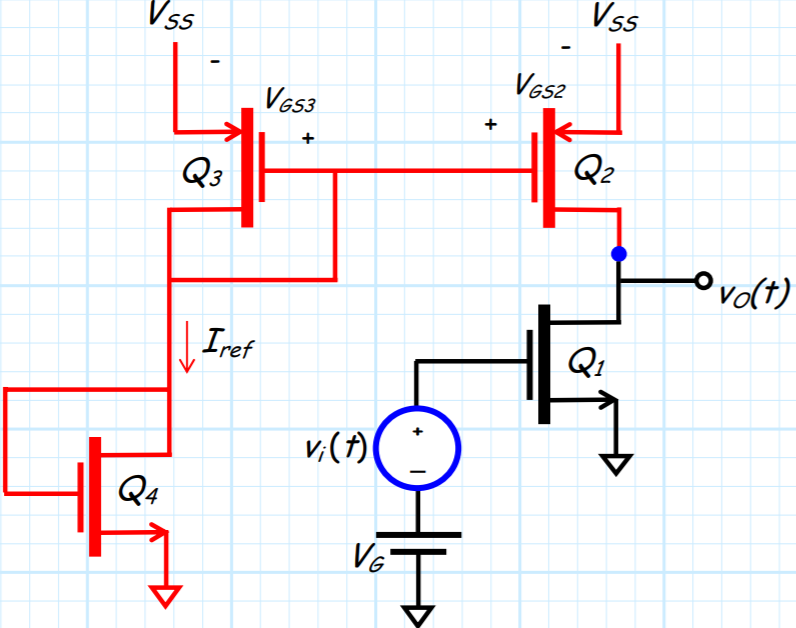
\includegraphics[width=\textwidth, height=14.35\baselineskip, keepaspectratio=true]{ds1}
\end{center}
\switchcolumn
\section{Problem 19.16-11.a.1: } 
\subsection{Design}

Design the all MOS inverter to bias the output at $\frac{V_{SS}}{2}$ when the input is at $\frac{V_{SS}}{2}$. Assume $V_{SS} = 5V$, $V_{TP} = -1V$, $V_{TN} = 1V$, $k_p = k_n = 50\mu A/V^2$, $i_D = 50\mu A$, $I_{ref} = 100\mu A$, and $V_g = 0.75V$.

At the bias, All transistors are in saturation.

\end{paracol}

\begin{align*}
   i_D
   &= \frac{k_n}{2}\frac{W}{L}_1(\frac{V_{SS}}{2} - V_{TN})^2
\\ \frac{W}{L}_1
   &= \frac{i_D}{\frac{k_n}{2}(\frac{V_{SS}}{2} - V_{TN})^2}
    = \frac{50\mu A}{\frac{50\mu A/V^2}{2}(\frac{5V}{2} - 1V)^2}
    = 0.8889
\\ i_D
   &= \frac{k_p}{2}\frac{W}{L}_2(V_{SS} - V_g + V_{TP})^2
\\ \frac{W}{L}_2
   &= \frac{i_D}{\frac{k_p}{2}(V_{SS} - V_g + V_{TP})^2}
    = \frac{50\mu A}{\frac{50\mu A/V^2}{2}(5V - 0.75V - 1V)^2}
    = 0.189
\\ I_{ref}
   &= \frac{k_p}{2}\frac{W}{L}_3 (V_{SS} - V_G + V_{TP})^2
\\ \frac{W}{L}_3
   &= \frac{I_{ref}}{\frac{k_p}{2}(V_{SS} - V_G + V_{TP})^2}
 	= \frac{100\mu A}{\frac{50\mu A/V^2}{2}(5V - 0.75V - 1V)^2}
	= 0.379
\\ I_{ref}
   &= \frac{k_n}{2}\frac{W}{L}_4 (V_G - V_{TN})^2
\\ \frac{W}{L}_4
   &= \frac{I_{ref}}{\frac{k_n}{2}(V_G - V_{TN})^2}
	= \frac{100\mu A}{\frac{50\mu A/V^2}{2}(0.75V - 1V)^2}
	= 64
\end{align*}

The circuit was designed with the following width ratios: $\frac{W}{L}_1 = 0.8889, \frac{W}{L}_2 = 0.189, \frac{W}{L}_3 = 0.379, \frac{W}{L}_4 = 64$.

This problem should demonstrate a basic ability to manipulate, design, and analyse MOSFET based logic gates. 

\textit{I have neither given nor received unauthorized assistance on this assignment.}


\end{raggedright}
\end{document}
